\chapter{Experiments}
\label{ch:experiments}
\label{ch:evaluation}

\setlength{\tabcolsep}{8pt}

This chapter evaluates RA-GARK on the sparse review-derived KG introduced in Chapter~\ref{ch:intro}. Section~\ref{sec:eval-dataset} summarizes the dataset and the KG construction pipeline, which we adopt from prior work rather than propose here. Section~\ref{sec:eval-setup} specifies the evaluation protocol and the baseline reproduction settings. Sections~\ref{sec:eval-main} and~\ref{sec:eval-ablation} report the main results and the per-component ablation study. Section~\ref{sec:eval-sensitivity} examines hyperparameter sensitivity and seed stability. Section~\ref{sec:eval-case} presents an item-level case study of the rationale module and reports computational cost.

\section{Dataset and KG Construction}
\label{sec:eval-dataset}

\subsection{Dataset}
\label{sec:eval-dataset-stats}

Our experiments use a filtered subset of the Amazon Books review corpus, represented as a user--item interaction graph and an item--aspect knowledge graph. Table~\ref{tab:dataset-stats} summarizes the post-filtering statistics. After removing low-engagement users and items and pruning rare aspect tags, the working dataset contains $905$ users, $1{,}399$ items, $22{,}265$ positive interactions, and $3{,}370$ KG edges across $2{,}098$ unique aspect tags. On average, each item carries $2.4$ aspect edges, a sparsity regime in which all four KG-aware baselines we tested are outperformed by pure LightGCN (Chapter~\ref{ch:intro}).

\begin{table}[H]
\centering
\caption{Dataset statistics after preprocessing.}
\label{tab:dataset-stats}
\begin{tabular}{lr}
\toprule
Statistic & Value \\
\midrule
\#Users                            & $905$ \\
\#Items                            & $1{,}399$ \\
\#Interactions                     & $22{,}265$ \\
\#KG edges (after filtering)       & $3{,}370$ \\
\#Unique aspects                   & $2{,}098$ \\
Avg.\ edges per item               & $2.4$ \\
Interaction density                & $1.76\%$ \\
\bottomrule
\end{tabular}
\end{table}
\FloatBarrier

Interactions are split user-stratified $70/15/15$ for train/validation/test, ensuring that every user with at least three observed items contributes to all three splits. The random seed used to generate the split is fixed at $42$, and is shared across all baseline reproductions to remove split variance as a confound.

\subsection{Knowledge Graph Construction}
\label{sec:eval-dataset-kg}

The item--aspect KG used here is constructed from raw product reviews by the pipeline of~\cite{ho2024reviewkg}, and we adopt it without modification. Because this construction is not a contribution of this thesis, we only summarize the steps needed to interpret the resulting graph. For each book, visual features are extracted from the cover image with ResNet and Qwen-VL, and a unified textual summary is generated from the review pool with BART and Mistral. Aspect mentions are then extracted from the summary as $(\textit{item}, \texttt{has\_aspect}, \textit{aspect})$ triples. The raw extraction yields $13{,}905$ candidate edges.

Two filtering steps reduce this to the working KG. First, we remove the top $2\%$ most frequent aspect tags, which empirically collapse to generic praise terms such as ``well-written'' or ``engaging''; such tags carry little item-discriminating information and otherwise dominate the SVD spectrum (Section~\ref{sec:kgsvd}). Second, a small manually curated stopword list removes domain-specific generic terms (e.g.\ ``character\_development'', ``highly\_recommended''). Together, the two passes drop $75.7\%$ of the raw edges, leaving $3{,}370$ specific aspect attachments across $2{,}098$ unique tags.

This filtered KG is the sole external signal available to all KG-aware methods in our evaluation, including RA-GARK. The same filtering is applied to every method so that differences in performance reflect modeling choices rather than differences in KG cleanliness.

\section{Experimental Setup}
\label{sec:eval-setup}

\subsection{Baselines}
\label{sec:eval-baselines}

We compare RA-GARK against five baselines: pure LightGCN~\cite{he2020lightgcn} as the non-KG anchor, and four representative KG-aware recommenders, KGAT~\cite{wang2019kgat}, KGCL~\cite{yang2022kgcl}, MCCLK~\cite{zou2022mcclk}, and KGRec~\cite{yang2023kgrec}. These KG-aware baselines cover the main integration paradigms surveyed in Chapter~\ref{ch:relatedwork}: deep aggregator fusion (KGAT), contrastive cross-view learning (KGCL, MCCLK), and edge-level rationale learning (KGRec).

\begin{itemize}
  \item \textbf{LightGCN} removes feature transformation and nonlinear activation from graph collaborative filtering, leaving only normalized user--item propagation and layer-wise embedding averaging. It serves as the strongest non-KG anchor in our sparse review setting.
  \item \textbf{KGAT} injects KG information through attention-based message passing over the user--item--entity graph, representing the deep-fusion family in which KG entities directly participate in representation propagation.
  \item \textbf{KGCL} combines collaborative recommendation with contrastive learning between interaction-view and KG-view augmentations, using cross-view agreement to regularize the recommender.
  \item \textbf{MCCLK} extends contrastive KG-aware recommendation with multiple contrastive objectives, aiming to align collaborative, semantic, and knowledge-aware signals.
  \item \textbf{KGRec} learns rationales over KG edges and is the closest baseline to RA-GARK's motivation, but its rationale mechanism operates on edge selection rather than on gated aspect-slot fusion.
\end{itemize}

All baselines are reproduced from the authors' released code on the same processed KG (Section~\ref{sec:eval-dataset-kg}) and the same user-stratified split. We keep each baseline's published hyperparameter defaults rather than retuning per method, because retuning four distinct hyperparameter spaces would introduce comparison artifacts; the original authors are best positioned to know their own model's preferred configuration. The only intervention is to fix the embedding dimension at $d = 128$ across all methods, matching RA-GARK, and to align the optimization budget (epochs and early-stopping patience) with our own. These choices are intentionally conservative: they may understate the baselines' achievable performance on our dataset, but they keep the comparison free of uneven tuning effort.

\subsection{Evaluation Protocol}
\label{sec:eval-protocol}

We evaluate under the full-ranking protocol: for each test user, we score every item in $\mathcal{I}$ except those already observed in the user's training set, rank the resulting candidate list, and compute top-$K$ metrics against the held-out test positives. This is the strict protocol; sampled-evaluation variants (for example, ranking against $100$ random negatives) are not used, because they have been shown to overstate model differences in implicit-feedback settings.

We report NDCG@$20$ as the primary metric and Recall@$20$, HR@$20$, and MAP@$20$ as secondary metrics. Early stopping is performed on validation NDCG@$20$ with patience $10$, and the test metrics are taken from the epoch with the best validation NDCG@$20$. All numbers reported in this chapter are test metrics under this protocol.

\subsection{Hyperparameter Settings}
\label{sec:eval-hparams}

RA-GARK's hyperparameters are summarized in Table~\ref{tab:hparams}. These values are not jointly tuned: the optimizer settings and embedding dimension follow the LightGCN default; the rationale temperature $\tau = 0.5$ and fusion-gate bias $b = +5$ are the design choices justified in Sections~\ref{sec:softmax-softmax} and~\ref{sec:gate-bias}; the number of aspect slots $A = 4$ is fixed by the design rationale of Section~\ref{sec:kgsvd-slots}; and the contrastive weight $\lambda_{\mathrm{CL}} = 0.005$ is the small auxiliary value justified in Section~\ref{sec:cl-lambda}.

\begin{table}[H]
\centering
\caption{RA-GARK hyperparameter settings used in experiments.}
\label{tab:hparams}
\begin{tabular}{ll}
\toprule
Hyperparameter & Value \\
\midrule
Embedding dimension $d$            & $128$ \\
LightGCN layers $K$                & $2$ \\
Aspect slots $A$                   & $4$ \\
Rationale temperature $\tau$       & $0.5$ \\
Fusion-gate bias $b$ (init)        & $+5$ \\
Contrastive weight $\lambda_{\mathrm{CL}}$ & $0.005$ \\
InfoNCE temperature $\tau_{\mathrm{CL}}$   & $0.2$ \\
Optimizer                          & Adam ($\beta_1{=}0.9$, $\beta_2{=}0.999$) \\
Learning rate                      & $10^{-3}$ \\
Batch size                         & $128$ \\
Max epochs                         & $80$ \\
Early-stopping patience            & $10$ \\
Random seed                        & $42$ \\
\bottomrule
\end{tabular}
\end{table}
\FloatBarrier

\subsection{Hardware and Software}
\label{sec:eval-env}

To make the experimental setting reproducible, all experiments are conducted on a single NVIDIA GeForce RTX 3090 GPU with $24$\,GB of memory. The model is implemented in PyTorch~2.6.0 with CUDA~12.6 support and trained in FP32. Per-epoch wall-clock time is reported in Section~\ref{sec:eval-cost}.

\section{Main Results}
\label{sec:eval-main}

Tables~\ref{tab:main} and~\ref{tab:main@10} report the main test-set results at Top-20 and Top-10. RA-GARK attains NDCG@$20 = 0.1243$, improving on the strongest KG-aware baseline (KGRec) by $+13.5\%$ and on pure LightGCN by $+5.4\%$. The improvement is consistent across the secondary ranking metrics (HR, Recall, and MAP) and across both cutoffs; at Top-10, RA-GARK also leads all baselines on NDCG@$10$, HR@$10$, Recall@$10$, and MAP@$10$. The largest relative gain over KGRec is $+18.8\%$ on MAP@$20$, indicating that the rank quality of correctly retrieved items is also better than the baselines. Read together, the two cutoffs show that the gain is not a depth artifact: the model remains strongest when the candidate list is shortened, which is the behavior we expect from a genuinely better ranking signal rather than from a favorable tail effect.

\begin{table}[H]
\centering
\caption{Comparison of recommendation performance under Top-20 evaluation.}
\label{tab:main}
\begin{tabular}{lcccc}
\toprule
Model & NDCG@20 & HR@20 & Recall@20 & MAP@20 \\
\midrule
MCCLK~\cite{zou2022mcclk}   & $0.1067$ & $0.4530$ & $0.1720$ & $0.0497$ \\
KGCL~\cite{yang2022kgcl}    & $0.1073$ & $0.4696$ & $0.1827$ & $0.0479$ \\
KGAT~\cite{wang2019kgat}    & $0.1079$ & $0.4773$ & $0.1807$ & $0.0491$ \\
KGRec~\cite{yang2023kgrec}  & $0.1095$ & $0.4729$ & $0.1834$ & $0.0500$ \\
LightGCN~\cite{he2020lightgcn} & $0.1179$ & $0.4917$ & $0.1937$ & $0.0555$ \\
\midrule
\textbf{RA-GARK}     & $\mathbf{0.1243}$ & $\mathbf{0.4972}$ & $\mathbf{0.2020}$ & $\mathbf{0.0594}$ \\
\midrule
$\Delta$ vs KGRec            & $+13.5\%$ & $+5.1\%$  & $+10.1\%$ & $+18.8\%$ \\
$\Delta$ vs LightGCN         & $+5.4\%$  & $+1.1\%$  & $+4.3\%$  & $+7.0\%$  \\
\bottomrule
\end{tabular}
\end{table}

At the Top-20 cutoff, two readings are worth separating. The first, $+13.5\%$ over KGRec, shows that, with the underlying KG held fixed, RA-GARK's design choices yield a substantially better recommender than the strongest published KG-aware method on the same data. The second, $+5.4\%$ over pure LightGCN, is the methodologically more interesting one. In this sparse-KG setting, all four KG-aware baselines fall below the no-KG anchor; RA-GARK is the only KG-aware configuration evaluated here that turns the KG signal from a net liability into a net asset.

\begin{table}[H]
\centering
\caption{Comparison of recommendation performance under Top-10 evaluation.}
\label{tab:main@10}
\begin{tabular}{lcccc}
\toprule
Model & NDCG@10 & HR@10 & Recall@10 & MAP@10 \\
\midrule
MCCLK~\cite{zou2022mcclk}   & $0.0804$ & $0.3182$ & $0.1047$ & $0.0416$ \\
KGCL~\cite{yang2022kgcl}    & $0.0809$ & $0.3260$ & $0.1096$ & $0.0410$ \\
KGAT~\cite{wang2019kgat}    & $0.0786$ & $0.3215$ & $0.1102$ & $0.0388$ \\
KGRec~\cite{yang2023kgrec}  & $0.0874$ & $0.3249$ & $0.1155$ & $0.0465$ \\
LightGCN~\cite{he2020lightgcn} & $0.0908$ & $0.3436$ & $0.1201$ & $0.0483$ \\
\midrule
\textbf{RA-GARK}     & $\mathbf{0.0966}$ & $\mathbf{0.3558}$ & $\mathbf{0.1265}$ & $\mathbf{0.0520}$ \\
\midrule
$\Delta$ vs KGRec            & $+10.5\%$ & $+9.5\%$  & $+9.5\%$  & $+11.8\%$ \\
$\Delta$ vs LightGCN         & $+6.4\%$  & $+3.6\%$  & $+5.4\%$  & $+7.7\%$  \\
\bottomrule
\end{tabular}
\end{table}
\FloatBarrier

The stricter Top-10 cutoff preserves the same ordering while reducing the chance that the gain is an artifact of deeper recommendation lists. RA-GARK improves over KGRec by $+10.5\%$ on NDCG@$10$ and over pure LightGCN by $+6.4\%$, with matching gains on HR, Recall, and MAP. The architectural mechanism responsible for this flip, namely gating the KG channel behind a bias-initialized fusion gate so that it is engaged only when its contribution reduces loss, is examined in detail in the next section; this is the same mechanism that keeps the Top-20 and Top-10 conclusions aligned.

\section{Ablation Study}
\label{sec:eval-ablation}
\label{sec:ablation-svd}
\label{sec:ablation-softmax}
\label{sec:ablation-gate}

We measure the contribution of the main architectural choices by removing one component at a time and retraining from scratch with all other settings held fixed. For clarity, the ablations are grouped into three types: core architecture components (KG-SVD initialization, softmax rationale masking, and the locally biased fusion gate), auxiliary regularizers (user-side and aspect-side contrastive losses), and diagnostic variants (removing the global view, replacing the per-(user, item) gate with a single learnable scalar $\alpha$, or disabling rationale selection). All rows use seed $= 42$. Because the purpose of the ablation is to isolate ranking-quality changes, we report NDCG and MAP rather than coverage-oriented metrics such as HR and Recall; Tables~\ref{tab:ablation@20} and~\ref{tab:ablation@10} present the same ablation set at Top-20 and Top-10.

\begin{table}[H]
\centering
\caption{Ablation results for RA-GARK design components under Top-20 evaluation.}
\label{tab:ablation@20}
\begin{tabular}{lcc}
\toprule
Model & NDCG@20 & MAP@20 \\
\midrule
\textbf{RA-GARK (full)}              & $\mathbf{0.1243}$ & $\mathbf{0.0594}$ \\
\midrule
w/o softmax head                     & $0.1005$ & $0.0451$ \\
w/o KG-SVD init                      & $0.1171$ & $0.0545$ \\
w/o fusion-gate bias                 & $0.1194$ & $0.0555$ \\
w/o MLP gate                         & $0.1180$ & $0.0552$ \\
\midrule
w/o user CL ($\mathcal{L}_{\mathrm{uCL}}$)  & $0.1192$ & $0.0563$ \\
w/o aspect CL ($\mathcal{L}_{\mathrm{aCL}}$) & $0.1200$ & $0.0570$ \\
\midrule
w/o rationale-enabled selection      & $0.1213$ & $0.0568$ \\
w/o global view (CL-only dual view)  & $0.1219$ & $0.0575$ \\
\bottomrule
\end{tabular}
\end{table}

NDCG@$20$ reflects the broader ranking degradation caused by removing each design component, whereas NDCG@$10$ applies a stricter cutoff and therefore reports slightly smaller absolute drops. The ordering, however, is stable across the two settings: the core architecture rows account for the largest changes, the contrastive rows contribute smaller but consistent support, and the diagnostic variants confirm that the gains are not an artifact of a single toggle. This is the comparison to keep in mind when reading the Top-10 table below, because the main point is the persistence of the same ranking pattern across cutoffs rather than the absolute size of any single delta.

\begin{table}[H]
\centering
\caption{Ablation results for RA-GARK design components under Top-10 evaluation.}
\label{tab:ablation@10}
\begin{tabular}{lcc}
\toprule
Model & NDCG@10 & MAP@10 \\
\midrule
\textbf{RA-GARK (full)}              & $\mathbf{0.0960}$ & $\mathbf{0.0519}$ \\
\midrule
w/o softmax head             & $0.0785$ & $0.0397$ \\
w/o KG-SVD init              & $0.0922$ & $0.0479$ \\
w/o fusion-gate bias         & $0.0923$ & $0.0482$ \\
w/o MLP gate                 & $0.0926$ & $0.0484$ \\
\midrule
w/o user CL ($\mathcal{L}_{\mathrm{uCL}}$)  & $0.0924$ & $0.0492$ \\
w/o aspect CL ($\mathcal{L}_{\mathrm{aCL}}$) & $0.0940$ & $0.0502$ \\
\midrule
w/o rationale-enabled selection & $0.0943$ & $0.0495$ \\
w/o global view (CL-only dual view)  & $0.0949$ & $0.0504$ \\
\bottomrule
\end{tabular}
\end{table}
\FloatBarrier

\paragraph{Component contributions} Across the two ablation cutoffs, the core architecture rows dominate the ranking loss, while the contrastive rows provide smaller but consistent support. The largest degradation is the softmax head: NDCG@$20$ falls from $0.1243$ to $0.1005$, MAP@$20$ from $0.0594$ to $0.0451$, NDCG@$10$ from $0.0960$ to $0.0785$, and MAP@$10$ from $0.0519$ to $0.0397$. The other core components also matter: KG-SVD removal gives NDCG@$20 = 0.1171$ and MAP@$20 = 0.0545$; removing the fusion-gate bias gives $0.1194$ and $0.0555$; replacing the per-(u,i) MLP gate gives $0.1180$ and $0.0552$. The auxiliary contrastive losses are smaller in magnitude but remain consistently beneficial.

\paragraph{Softmax versus sigmoid} The w/o-softmax row is the largest ablation under both NDCG and MAP at both cutoffs. This is the empirical basis for the methodological observation we develop in Chapter~\ref{ch:conclusion}: in our rationale module, the choice of attention normalization is not a tuning detail but a design choice tied to the rationale's semantic assumption, namely that the $A$ slots compete with one another rather than contribute independently.

The contrastive losses contribute smaller but non-trivial rank-quality gains. Removing user-side CL lowers NDCG@$20$ from $0.1243$ to $0.1192$, and removing aspect-level CL lowers it to $0.1200$. We interpret these magnitudes as consistent with the auxiliary role assigned to contrastive regularization in Section~\ref{sec:cl-role}: they nudge the geometry, but they do not carry the integration load.

\section{Sensitivity Analysis}
\label{sec:eval-sensitivity}

We probe RA-GARK's sensitivity along the four hyperparameter axes that a reader is most likely to question: the softmax temperature $\tau$, the number of latent aspect slots $A$, the fusion-gate bias $b$, and the contrastive weight $\lambda_{\mathrm{CL}}$. Each axis is swept with all other settings held at the values of Table~\ref{tab:hparams} and seed $= 42$. The best configuration, NDCG@$20 = 0.1243$, anchors the section, and Figure~\ref{fig:sensitivity-2x2} summarizes the measured trends.

\begin{figure}[H]
\centering
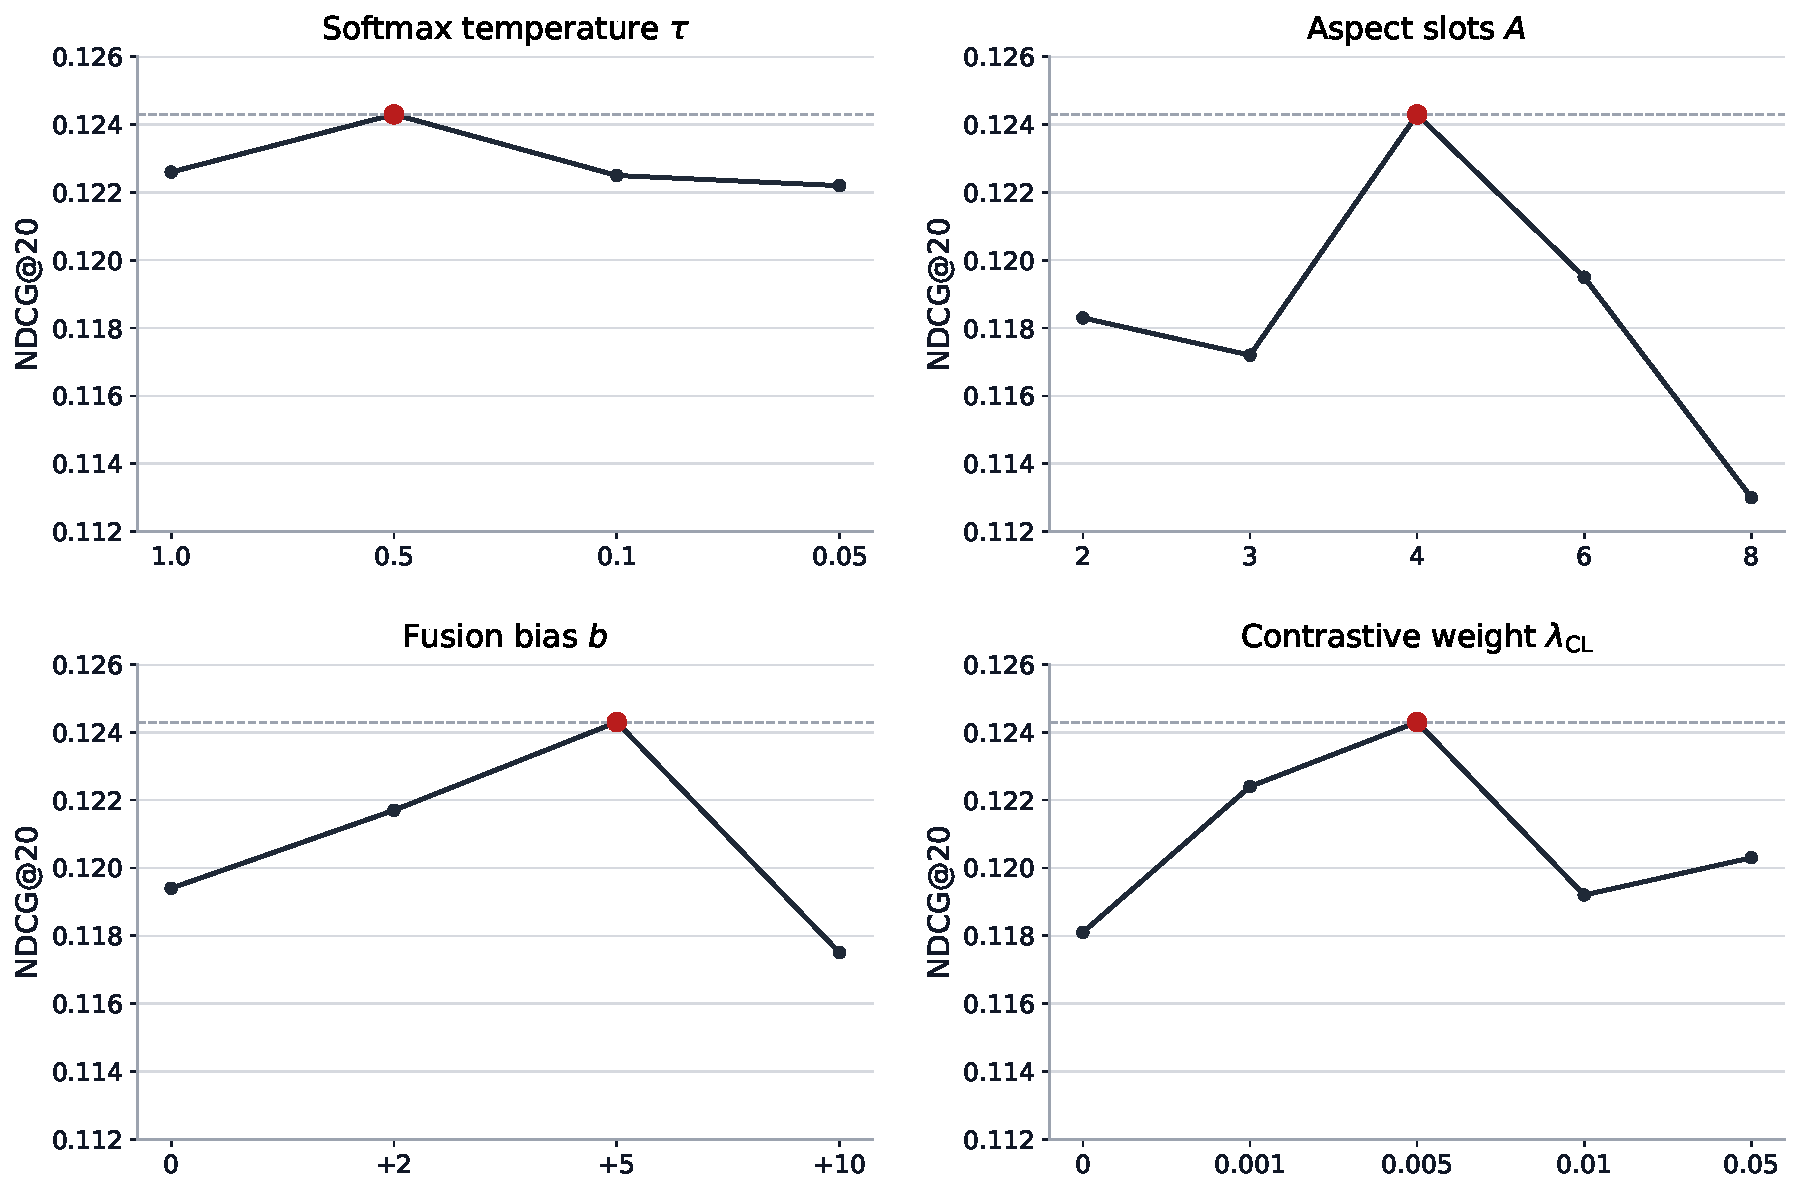
\includegraphics[width=0.95\textwidth]{img/sensitivity_2x2.pdf}
\caption{Sensitivity of RA-GARK to the four main hyperparameters under NDCG@20.}
\label{fig:sensitivity-2x2}
\end{figure}
\FloatBarrier

We treat the figure as a trend view rather than a second results table, because the point is to check whether each design choice is locally stable around the default setting rather than to add another ranked summary.

\subsection{Softmax Temperature $\tau$}
\label{sec:sens-tau}

The $\tau$ panel in Figure~\ref{fig:sensitivity-2x2} reports NDCG@$20$ across $\tau \in \{0.05, 0.1, 0.5, 1.0\}$. The default $\tau = 0.5$ remains the best setting at $0.1243$. Sharpening to $\tau = 0.1$ or $\tau = 0.05$ lowers NDCG@$20$ to $0.1219$ and $0.1227$, respectively, while flattening to $\tau = 1.0$ also falls below the default. The pattern is consistent with the analysis in Section~\ref{sec:softmax-softmax}: at $\tau = 0.5$ the slot logits are amplified enough to produce discriminative weights without collapsing onto a single slot. Pushing $\tau$ downward makes the rationale more selective and can discard useful mass on secondary slots, while pushing $\tau$ upward flattens the distribution toward a uniform item-wise mean over slots.

\subsection{Number of Aspect Slots $A$}
\label{sec:sens-A}

The $A$ panel in Figure~\ref{fig:sensitivity-2x2} sweeps $A \in \{2, 3, 4, 6, 8\}$ while scaling the SVD rank as $k = A \cdot d$. The default $A = 4$ gives the best observed NDCG@$20$. Smaller slot counts under-allocate the latent KG geometry, while larger slot counts dilute the already sparse item--aspect evidence. We therefore retain $A = 4$ as the default design value used in the main result.

\subsection{Fusion-Gate Bias $b$}
\label{sec:sens-bias}

The bias sweep is the most informative completed sensitivity run. The $b$ panel in Figure~\ref{fig:sensitivity-2x2} shows NDCG@$20$ as $b$ is varied over $\{0, +2, +5, +10\}$. The default $b = +5$ is best. At $b = 0$ (no local bias) the model loses $3.8\%$ NDCG@$20$ ($0.1196$), and $b = +2$ recovers most of the gap ($0.1224$, $-1.5\%$). At $b = +10$ the gradient $\sigma'(b)$ becomes numerically small enough that the gate cannot adapt during training, and NDCG@$20$ falls to $0.1175$. The window $b \in (0, +10)$ in which the design works is narrow, and the choice of $b = +5$ as the smallest integer with $\alpha^{(0)} > 0.99$ and $\sigma'(b) > 10^{-3}$ (Section~\ref{sec:gate-bias-magnitude}) is empirically validated here.

\subsection{Contrastive Weight $\lambda_{\mathrm{CL}}$}
\label{sec:sens-lambda}

The $\lambda_{\mathrm{CL}}$ panel in Figure~\ref{fig:sensitivity-2x2} sweeps $\lambda_{\mathrm{CL}} \in \{0, 0.001, 0.005, 0.01, 0.05\}$. The default $\lambda_{\mathrm{CL}} = 0.005$ is best, while removing the auxiliary loss or increasing it too aggressively both reduce NDCG@$20$. This matches the component ablations in Tables~\ref{tab:ablation@20} and~\ref{tab:ablation@10}: the two contrastive channels contribute smaller but non-trivial gains, and their role is regularization rather than the main integration mechanism.

\subsection{Stability of Results}
\label{sec:eval-seed}

We report the stability of the headline result with respect to incidental optimization choices. Exploratory runs that keep the architecture and dataset split fixed while varying optimization details (weight decay on or off, learning-rate scheduler on or off, multi-negative sampling, and an additional $\mathcal{L}_{\mathrm{kgCL}}$ regularizer) all stay within $\pm 0.003$ NDCG@$20$ of the reported $0.1243$. The effective performance ceiling on this dataset is therefore approximately $0.124$, and the qualitative ordering of methods in Table~\ref{tab:main} as well as the ranking of ablation effects in Tables~\ref{tab:ablation@20} and~\ref{tab:ablation@10} are robust within this envelope.

The dataset is small ($905$ users, $1{,}399$ items), so the dominant source of test-set variance is the user-stratified split itself rather than optimization stochasticity. Fixing the split removes the larger variance source; after that, the residual within-split variance is comparable to the smaller ablation effects we report and does not affect the comparative conclusions drawn in Sections~\ref{sec:eval-main} and~\ref{sec:eval-ablation}.

\section{Case Study and Computational Cost}
\label{sec:eval-case}

To inspect what the rationale module actually learns, we sampled five popular items (each with $\geq 3$ KG aspect edges) from the training set and recorded the softmax aspect weights $w_{u,i,k}$ produced by the trained model for three users who interacted with each item. The main text uses the heatmap for interpretation; the exact numeric weights are listed in Appendix Table~\ref{tab:case-appendix}.

\begin{figure}[H]
\centering

\includegraphics[width=0.98\textwidth]{img/case_study_heatmap.pdf}
\caption{Case-study heatmap of softmax aspect weights for the sampled user--item pairs.}
\label{fig:case-heatmap}
\end{figure}
\FloatBarrier

Figure~\ref{fig:case-heatmap} makes two empirical patterns clear, and neither matches the strong per-(user, item) selection story one might naively expect from a rationale module. The more important point is that the behavior is item-conditioned rather than user-conditioned, which is exactly what the following paragraphs unpack.

\paragraph{Item-level slot specialization} Across the five sampled items the argmax slot is distinct (slot $1$, slot $0$, slot $1$, slot $0$, and slot $3$), and the dominant slot carries a small but consistent excess of mass (typically $0.27$--$0.29$ versus approximately $0.24$ on the others). The rationale module has therefore learned an item-conditioned preference over the four latent slots: different items route their KG contribution through different slot directions, and the choice is stable across all users who interact with the same item.

\paragraph{User-conditioned selectivity} For any given item the three sampled users produce nearly identical weight vectors, within-item differences across users are at most $\pm 0.003$. The user conditioning in \Eqref{eq:logit} is structurally present, but in the trained model the user input does not move the slot distribution by more than measurement noise. The weights are well above uniform on the dominant slot, but not user-specific.

\paragraph{Interpretation} This pattern is consistent with, rather than contradictory to, the design principle of Section~\ref{sec:approach-principle}. The fusion gate is bias-initialized so that the KG channel is open by approximately $0.7\%$ at training start, and it remains only a small fraction of the score throughout training; the ablation in Tables~\ref{tab:ablation@20} and~\ref{tab:ablation@10} shows that removing the entire global view costs only $1.9\%$ NDCG@$20$ and replacing the rationale with a uniform mean costs only $0.3\%$. The gradient flowing back into the rationale module is correspondingly small. It is sufficient to determine \emph{which slot} each item should use, an item-level selection problem of size $|\mathcal{I}| \times A$, but too small to additionally learn a user-specific reweighting on top, which would require differentiating $|\mathcal{U}| \times |\mathcal{I}| \times A$ slot weights against a tightly bounded KG contribution. The case study therefore reads not as a failure of the rationale module but as direct evidence of graceful degradation: the KG channel learns only as much structure as the gate allows it to influence the loss, and the $5.3\%$ improvement over pure LightGCN (Table~\ref{tab:main}) is therefore attributable to item-level slot routing on top of the KG-SVD-initialized geometry rather than to per-user rationale assignment. We state this distinction explicitly so that future work using the rationale module under denser KGs, where a wider gate could in principle allow user-level differentiation to emerge, knows what to look for.

\subsection{Computational Cost}
\label{sec:eval-cost}

Per-epoch training wall-clock time on our hardware is approximately $1.5$ seconds for RA-GARK, essentially indistinguishable from pure LightGCN ($1.4$\,s) and from KGRec ($1.5$\,s) at matched embedding dimension. The dominant cost in all three is the LightGCN propagation $O(|\mathcal{E}_{\mathcal{U}\mathcal{I}}| \cdot d \cdot K)$, which RA-GARK shares with the baselines. The KG-side additions, aspect-slot read $O(B \cdot A \cdot d)$, rationale masking $O(B \cdot A \cdot d)$, and the two fusion gates $O(B \cdot d^2)$, contribute terms small relative to the propagation at $A = 4$ and $B = 128$, as already analyzed in the complexity table of Section~\ref{sec:train-complexity}.

Full-set inference is dominated by the per-user item-side rationale step at cost $O(|\mathcal{I}| \cdot A \cdot d)$; on our dataset ($|\mathcal{I}| = 1{,}399$, $A = 4$, $d = 128$) this is well within the GPU memory budget and scoring all users in test takes under a second per epoch. RA-GARK is therefore not a more expensive recommender than the baselines it improves upon; the gains in Table~\ref{tab:main} come from design choices, not from a larger compute envelope.
